\chapter{Ontology guided approach to retrieving medically-relevant web images: application on retrieving disease manifestation images}\label{image2}

\section{Motivation}
Towards the goal of constructing a patient-oriented health image base,
we propose a content-based image retrieval (CBIR) method
to retrieving disease manifestation images from the web.
The image retrieval task is highly challenging, since disease manifestation
images contain diverse objects and complex backgrounds.
For example, the positive examples of ``hand,
foot, and mouth disease" may contain infected feet,
hands, mouths, or tongues. The body parts are in
different positions and sizes, and more
than one infected body part may appear in one
single image. To collect disease images from the
web, we need to analyze the image at the object
level at the minimal cost of manual effort.
%\begin{figure}[htb!]
%\vspace{0em}
%\begin{center}
%\includegraphics[width=0.8\textwidth]{Chap2_handfootmouth.eps}
%\vspace {0em}\caption{Positive examples of images on hand, foot, and mouse disease.} \label{handfootmouth}
%\end{center}
%\vspace {0em}
%\end{figure}

Most CBIR systems apply machine learning approaches to
bridge the semantic gap between image content and users' interpretations \cite{datta2008image}.
These approaches include supervised classification \cite{chapelle1999support},
similarity-based clustering \cite{li2008real}, semi-supervised
co-training \cite{feng2004bootstrapping}, and active learning based on relevant feedback \cite{tong2001support}.
A few methods incorporated additional information to improve
retrieval precision. For example, Deserno {\it et al} exploited
figure types and panel numbers to retrieve literature figures \cite{deserno2009content}.
Muller {\it et al} summarized the retrieval methods for integrating
texts with image content \cite{muller2012overview}.
Simpson {\it et al} combined natural language
and image processing to map regions in CT scans to concepts
in RadLex ontology, which was automatically extracted
from image captions \cite{simpson2012towards}.
Deng {\it et al} used semantic prior knowledge
to retrieve similar images \cite{deng2011hierarchical}. One particularly relevant
method of reducing human effort in health image collection is
the bootstrap image classification method \cite{chen2012semi}. This approach uses
one positive sample as the ``seed" to iteratively retrieve more
positive images, and thus is appropriate for large-scale image
collection. Although this approach effectively collects human
organ and drug images, it has limited precision for disease
images \cite{chen2012semi}. Because web images are highly heterogeneous, our
task requires supervision of the training data to ensure good
precision. However, traditional supervised methods need a training
image set for each disease, thus will not scale up
when the number of disease terms is large.

To solve the scalability problem, we propose an ontology-guided
organ detection method to collect disease manifestation
images from the web. Based on observation, we assume that
most disease manifestation images contain abnormal human
body parts, such as eyes, ears, and hands, which show visible
disease symptoms. Therefore, our approach uses the existence
of these body parts to discriminate between images of disease
and non-disease images. Instead of training a classifier for each
disease, we pretrain a set of organ detectors, each of which
detects one target organ. When retrieving images for a given
disease, we extract the disease-organ semantic relationships
from ontologies, and use the corresponding detectors to detect
associated organs from web images.

Our method has two major advantages. First, we require much
fewer training data than the standard supervised method, which
trains a classifier for each disease, because we reuse organ detectors
across diseases. For example, 428 diseases in the UMLS
record eyes. Instead of training 428 classifiers, one for each
disease, we train one detector for ``eye" and reuse it to classify
428 types of eye disease images. Second, our approach achieves
high accuracy when disease images contain diverse manifestations
of different organs, such as images of ``hand, foot, and mouth
disease." For each disease, we use prior knowledge of disease-
organ associations as guidance to scan images at the object level.


\section{Data and methods}

Fig. {\ref{Chap2_system}}A shows the steps of the method. For a given disease, we first use the UMLS to determine what body parts the disease is manifested on. Then we use a set of pre-trained body part detectors, using state-of-the-art image features, to find the targets at multiple scales. Finally we combine the scanning results of each detector at all scales into high level features to classify the input images as relevant or irrelevant.
\begin{figure}[t]
\vspace{0em}
\centering
\includegraphics[width=\textwidth]{Chap2_system.eps}
\vspace {0em}\caption{(A) The Overview of disease image retrieval approach. We use the UMLS to determine the body part locations of disease manifestations and to select from a set of pre-trained body part detectors to filter Google search results into relevant and irrelevant images. Comparing to a supervised method that would require labeled training examples for each disease, we achieve high precision in image retrieval while reducing human effort to a minimum. (B) The structure of organ detectors. Our decision rule is based on multiple objects detectors at multiple scales. It is crucial to have multiple scales because some disease images have body parts occupying the entire frame, while others include a large portion of the background.}
\label{Chap2_system}
\vspace {0em}
\end{figure}


\subsection{Discovering target body parts}
For each target disease, we find its corresponding body parts through the UMLS semantic network relationship of ``has\_finding\_site". One body part is typically associated with at least hundreds of diseases; this fact shows that reusing common body part detectors across diseases can save a huge amount of human labeling effort. Each disease can have manifestations on multiple body parts:  among the diseases that involve the ``has\_finding\_site" relation in UMLS, around 15\% of them are located on more than one body parts. For such complex diseases, we will combine the detection results of multiple body parts into high level features to boost the retrieval precision.

Some diseases affect internal organs that are not directly visible in images. Nonetheless, symptoms on these organs can have direct manifestation on external body parts. We manually map part internal organs to their associated external body parts by using the ``isa" and ``part\_of" relationships in the UMLS. For example, the ``oral mucous membrane structure" is a part of the ``entire mouth region", which is a synonym of ``mouth" in the UMLS. Thus diseases having the symptoms in ``oral mucous membrane structure" are considered to be associated with ``mouth". In addition, some diseases are located on body parts that are too detailed according to the UMLS. We also manually map such body parts to the larger organs that contain them based on the ``part\_of" relationship. For example, ``upper eye lid" and ``lower eye lid" are parts of ``eye", therefore are mapped to ``eye". Diseases manifested on upper and lower eyelids then have ``eye" as the target body part.

\subsection{Detecting target body parts}
We develop a general human organ detection method, and adapt it to specific targets by tuning training data as well as parameters. Currently, we have trained detectors for eye, ear, lip/mouth, hand and foot, and reused them in retrieving images of a variety of diseases. The detectors are learned in a generic way and can be easily extended to other body parts.

Object detection is a fundamental problem in computer
vision. Approaches to object detection typically consist of two
major components: feature extraction and model construction.
Lowe developed the scale invariant feature transformation
(SIFT) as the image patch descriptor \cite{lowe1999object}.
Dalal and Triggs \cite{dalal2005histograms} proposed
the histograms of oriented gradients (HOG) for human
detection. These features have proved effective in object detection
applications. In addition, Zhang {\it et al} constructed a
bag-of-feature model to classify texture and object categories \cite{zhang2007local}.
Felzenszwalb {\it et al} developed a generic object detector with
deformable part models to handle significant variations in object
appearances \cite{felzenszwalb2010object}.


Fig. {\ref{Chap2_system}}B shows the structure of our organ detector. Each
detector $i (i=A, B…)$ detects one target organ using multiple
classifiers. Each classifier $C_{ij}$ scans the input image and searches
for the target at detection scale $j ( j=1, 2…)$. For example, if
detector $A$ is an eye detector and contains three classifiers, then
$C_{A1}$ decides if the full image is an eye, $C_{A2}$ scans the image with
a detection window to search for small eyes, and $C_{A3}$ searches
for eyes of an even smaller size. The organ detection results
${S_{A1}, S_{A2}, ..., S_{B1}, S_{B2}}$ are binary values and represent the
existence of each organ $\{A,B,\cdots\}$ at each detection scale $\{1,2,\cdots\}$.
We then combined these results into high-level features,
based on logic, to make final decisions about the input images.
We found that the accuracies of our simpler detection system
were comparable to that of Felzenszwalb et al \cite{felzenszwalb2010object}.



\subsubsection{Training organ detectors}
For all classifiers in each organ detector, the training samples
consisted of web images collected by Google. To collect positive
examples, we searched the six body part names as the keywords
and manually picked 200--300 images of the body part itself
with little background. Most positive examples are not medically
relevant, but contain different views of the body parts. To
collect negative images, we summarized the categories of objects
and backgrounds that often appear in the Google query results,
such as paper snapshots, animals, and buildings. Negative examples
were then collected by searching keywords such as ``research
paper," ``dog," and ``building." Five thousand images comprised
the negative training set. We used the same negative examples
for all the organ detectors.

We trained three standard soft margin support vector
machine (SVM) classifiers for each organ detector to detect
targets on three scales. In detector i, $C_{i1}$ was trained by full
training images. Since $C_{i2}$ and $C_{i3}$ search for targets with detection
windows, they used positive samples that were resized to
the window sizes, and randomly selected image patches of the
window sizes from negative samples. We extracted the HOG
features \cite{dalal2005histograms} from training images. The HOG is reminiscent of the
SIFT descriptor, but uses overlapping local contrast normalizations
for improved performance \cite{dalal2005histograms}. The window sizes of $C_{i2}$ and
Ci3 were empirically chosen as $64 \times 96$ pixels and $32 \times 48$ for
eye, lip/mouth, and hand detectors; and $96 \times 64$ and $48 \times 32$ for
foot and ear detectors. By browsing 100 eye disease images, we
found that images containing only very small target organs were
usually false positives, therefore did not train classifiers at any
smaller scale in order to maintain high retrieval precision.



\subsection{Combining detections for disease image classification}
We finally used the organ detection results that represent the
existence of affected organs as high-level features to classify the
input images into disease or non-disease categories. Ideally, if all
the classifiers behave in the same way and are independent, the
high-level combined feature might look like:
\begin{equation}\label{decision2}
y = ({S_{A1}} + {S_{A2}} + {S_{A3}}) + ({S_{B1}} + {S_{B2}} + {S_{B3}}) + ...,
\end{equation}
where $+$ is the `or' operation between binary values.

However, we found that such a simple combination had problems.
If the whole image itself is the target body part, it is
unlikely to contain the same target at smaller scales. If a body
part is detected at both the whole-image level and the finer
scales, the image is often a false positive. This may be partly due
to the incompleteness of the training samples or the challenge
of detection of small-scale objects. Rule \eqref{decision2} ignores this problem
and concludes that the result is positive if the classifiers at all
three scales are positive. As precision is more important for our
retrieval problem, we used the exclusive `or' operation to set
the decisions in such cases as negative, even though the recall
might be decreased.
Our final decision rule was as follows:
\begin{equation}\label{decision}
y = ({S_{A1}} \oplus ({S_{A2}} + {S_{A3}})) + ({S_{B1}} \oplus ({S_{B2}} + {S_{B3}})) + ...,
\end{equation}
where $\oplus$ is the exclusive `or' and $+$ is the `or' operation between binary values.

Comparison of the truth of \eqref{decision2} and \eqref{decision}
shows that the two equations make different decisions only
when the detection results are positive at both the whole-image
level and the finer levels, and then decision rule \eqref{decision} is more
desirable.




\section{Results}
We evaluated the proposed ontology-guided disease image
retrieval method for two kinds of image sets: (1) images of multiple
diseases that are located on the same body part, and (2)
images of diseases that are located on more than one body part,
in experiments A and B, respectively. All the test images were
top Google search results for the given disease term. We
excluded those images with either widths or heights smaller
than 128 to ensure image quality. Also, to apply the organ
detectors with the selected detection window sizes, we resized
all test images such that both their widths and heights were
between 128 and 256. For evaluation purposes, the test images
were labeled by three human evaluators. Since performance
depends on the ground-truth labeling, a majority vote was used
among individual evaluators. The average agreement rate among
the three evaluators was 92\%.

\subsection{Single-organ disease classification}
Our method trained organ detectors by normal organ images.
Since the test images can be quite different from the training
images and much more diverse, we designed experiment A to
evaluate the performance of our method by comparing the
results with a supervised classification method. For each individual
disease, the supervised method trained a soft margin SVM
classifier using the actual disease images as training data, and
extracted the same HOG features.

This experiment repeatedly compared our object detection based
method with the supervised classification method on
2000 test images in three groups. Each group contains 10 sets
of eye, ear, and mouth/lip disease images, respectively. Our
method trains a single object detector to classify the 10 test sets
in each group. In contrast, the supervised method trains 10 different
classifiers for each disease, thus requiring 10 times more
human labeling effort. The methods compared their precisions,
recalls and F1 measures. Precision is the most important criterion
among the three, because our goal is to collect data for a
health image base, and we are more interested in the credibility
than the completeness of the images. Table \ref{eyeres} compares the performance
for eye disease images. The average positive percentage
of the 10 Google test image sets is 52.2\%. After using our
method, the average positive percentage of the retrieved images
was 79.1\%. For 9 out of 10 test sets, our method achieved precision
of between 70\% and 90\%. The precisions, recalls and F1
measures of our method were comparable ($p>0.1$) to those of
the supervised method for all the 10 test sets, even though our
method only needs one tenth of the manual labeling effort, by
reusing the organ detector across 10 diseases. In practice, our
method will be able to reuse the eye detector for far more than
10 eye diseases and further reduce human effort.

\setlength{\tabcolsep}{5.7pt}
\begin{sidewaystable}
\centering
\caption{Performance Comparison on Ten Eye Disease Image Test Sets.}\label{eyeres}
\renewcommand{\arraystretch}{1.3}
\begin{tabular}{cccccccc}
\hline
\multicolumn{2}{l}{Eye diseases} & \multicolumn{3}{l}{Object Detection Based Method} &
\multicolumn{3}{l}{Supervised Classification Method} \\ \hline
Disease CUI    &Disease Term & Precision & Recall & F1    & Precision & Recall & F1 \\ \hline
C0009363       & Coloboma    &{\b 0.750} &0.720   &0.735  & {\b 0.707}&0.746   &0.726 \\ \hline
C0013261&Duane retraction syndrome& 0.818& 0.400  &0.537  &0.779      &0.652   &0.710 \\ \hline
C0014236&Endophthalmitis     &0.852      & 0.697  &0.767  &0.817      &0.867   &0.841 \\ \hline
C0015397 &Disorder of eye    &0.882      &0.882   &0.882  &0.683      &0.700   &0.692 \\ \hline
C0015401 &Eye foreign bodies &0.826      &0.792   &0.809  &0.648      &0.687   &0.667 \\ \hline
C0015402 &Eye hemorrhage	 &0.692      &0.800   &0.742  &0.772      &0.821   &0.796\\ \hline
C0015404 &Bacterial eye infections	&0.706    &0.720  &0.713      &0.807   &0.864   &0.834\\ \hline
C0017601 &Glaucoma           &0.727 &0.800 &0.762 &0.821 &0.827 &0.824\\ \hline
C0025210 &Ocular melanosis &0.794 &0.540 &0.643 &0.723 &0.689 &0.706 \\ \hline
C0086543 &Cataract &0.862  &0.806 &0.833 &0.862 &0.913 &0.887\\ \hline
\multicolumn{2}{l}{Average}&0.791 &0.716 &0.742 &0.762 &0.777 &0.768 \\ \hline
\end{tabular}
\end{sidewaystable}

Also, we observed that the object detectors at smaller detection
scales tend to introduce more false-positive results. For eye
disease image retrieval, a finer detection scale yields decreasing
precision in 8 out of 10 test sets (Fig. \ref{Chap2_trend}A) and increasing
recall in all test sets (Fig. \ref{Chap2_trend}B). The second test set of Duane
retraction syndrome images has the lowest recall in all detection
scales. One possible reason is that many positive images in this
set contain eyes smaller than our detection window scales in
order to illustrate the eye movement disorder. Adding organ
detectors at smaller scales may increase the recall, but may also
introduce many false positives. Since precision is of more
importance, we stopped the object detection at the third detection
scale.
\begin{figure}[t]
\vspace{0em}
\centering
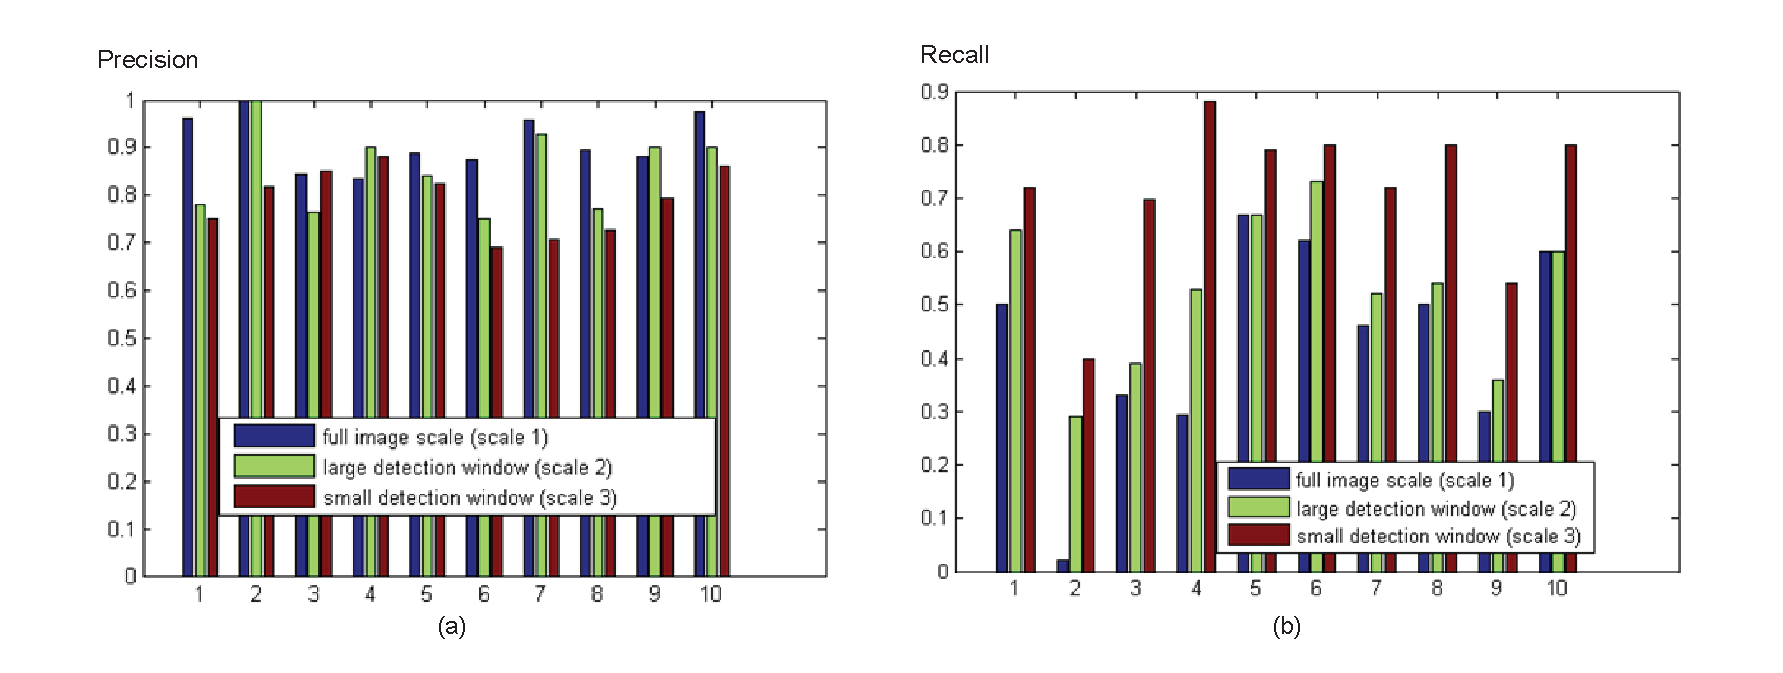
\includegraphics[width=\textwidth]{Chap2_trend}
\vspace {0em}\caption{(A) Trend for decreasing precision in finer scales. (B) Trend for increasing recall in finer scales.}
\label{Chap2_trend}
\vspace {0em}
\end{figure}



Table {\ref{earres}} and {\ref{mouthres}} show the results for ear and mouth/lip disease images. Our method achieved average precisions of
80.7\% and 84.2\%, while the baselines of test set quality were
43.4\% and 47.5\%, respectively. The three evaluation criteria in
table {\ref{earres}} are similar between the two methods ($p>0.1$), and the
average precision of our method for ear disease retrieval was
higher than that of the supervised method. In table \ref{mouthres}, our
method achieved around 6\% average higher precision than the
supervised method ($p=0.15$), at the cost of lower recall. One
possible reason is that the body parts in some mouth disease
images from the test sets are at very different angles and considerably
deformed.
\setlength{\tabcolsep}{5.7pt}
\begin{sidewaystable}
\centering
\caption{Performance Comparison on Ten Ear Disease Image Test Sets.}\label{earres}
\renewcommand{\arraystretch}{1.3}
\begin{tabular}{cccccccc}
\hline
\multicolumn{2}{l}{Ear diseases} & \multicolumn{3}{l}{Object Detection Based Method} &
\multicolumn{3}{l}{Supervised Classification Method} \\ \hline
Disease CUI    &Disease Term & Precision & Recall & F1    & Precision & Recall & F1 \\ \hline
C0008373	&Cholesteatoma&	0.794	&0.818&	0.806&	0.881&	0.953&	0.915\\ \hline
C0013446	&Acquired Ear Deformity&	1.000&	0.828&	0.906&	0.819&	0.863&	0.840\\ \hline
C0013449	&Ear Neoplasms	&0.875	&0.412&	0.560&	0.733	&0.567&	0.639\\ \hline
C0029877	&Ear Inflammation	&0.921&	0.778	&0.843	&0.822	&0.804	&0.813\\ \hline
C0154258	&Gouty tophi of ear	&0.792	&0.655&	0.717&	0.614	&0.470&	0.532\\ \hline
C0347354	&Benign neoplasm of ear	&0.571	&0.533&	0.552&	0.820	&0.497&	0.619\\ \hline
C0423576	&Irritation of ear	&0.733	&0.611	&0.667	&0.933	&0.607	&0.735\\ \hline
C0521833	&Bacterial ear infection&	0.786	&0.647&	0.710&	0.820	&0.670&	0.737\\ \hline
C0729545	&Fungal ear infection	&0.800	&0.696	&0.744&	0.728	&0.864	&0.791\\ \hline
C2350059	&Cancer of Ear&	0.800	&0.414&	0.545&	0.797	&0.699&	0.736\\ \hline
\multicolumn{2}{l}{Average}&0.807&	0.639	&0.705&	0.797	&0.699&	0.736\\ \hline
\end{tabular}
\end{sidewaystable}

\setlength{\tabcolsep}{5.7pt}
\begin{sidewaystable}
\centering
\caption{Performance Comparison on Ten Mouth/Lip Disease Image Test Sets.}\label{mouthres}
\renewcommand{\arraystretch}{1.3}
\begin{tabular}{cccccccc}
\hline
\multicolumn{2}{l}{Mouth/Lip diseases} & \multicolumn{3}{l}{Object Detection Based Method} &
\multicolumn{3}{l}{Supervised Classification Method} \\ \hline
Disease CUI    &Disease Term & Precision & Recall & F1    & Precision & Recall & F1 \\ \hline
C0007971	&Cheilitis	&0.846&	0.667&	0.746	&0.828&	0.893	&0.859\\ \hline
C0019345	&Herpes Labialis&0.900	&0.486	&0.632	&0.817	&0.953&	0.880\\ \hline
C0023761	&Lip Neoplasms	&0.909	&0.500	&0.645	&0.607	&0.553	&0.579\\ \hline
C0149637	&Carcinoma of lip	&0.952	&0.435	&0.597&	0.819	&0.906	&0.860\\ \hline
C0153932	&Benign neoplasm of the lip	&0.625	&0.333	&0.435	&0.833&	0.713	&0.769\\ \hline
C0158670	&Congenital fistula of lip	&0.700	&0.368&	0.483	&0.693	&0.800	&0.743\\ \hline
C0221264	&Cheilosis	&0.750	&0.577	&0.652	&0.813	&0.867	&0.839\\ \hline
C0267022	&Cellulitis of lip	&0.923	&0.600	&0.727	&0.810	&0.917	&0.860\\ \hline
C0267025	&Contact cheilitis	&0.950&	0.543	&0.691	&0.849	&0.943	&0.894\\ \hline
C0267032	&Granuloma of lip	&0.867	&0.500	&0.634&	0.721	&0.865&	0.786\\ \hline
\multicolumn{2}{l}{Average}&0.842	&0.501	&0.624&	0.779&	0.841	&0.807 \\ \hline
\end{tabular}
\end{sidewaystable}

\subsection{Multiple-organ disease classification}
Experiment B evaluated the performance of our method on 220
images of two diseases that are located on multiple organs.
Table {\ref{multiorgan}} shows that the precision of the proposed method on
both test sets was $>80\%$. Compared with the supervised
method, our method improved precision by more than 10\% in
these two cases. Since the proposed method is guided by the
semantic information of body part location, it can detect
various kinds of positive images, whereas the supervised method
does not make use of the high-level features that have greater
semantic meaning.

For hand, foot, and mouth disease, 42.9\%, 28.6\%, and
37.1\% of the positive images in the test set contained a hand,
foot, and mouth, respectively. A few positive images contained
two or three body parts at the same time. The hand, foot, and
lip/mouth detectors contributed to finding 28.6\%, 14.3\%, and
28.6\% of the total positive images. For Ascher's syndrome,
67.9\% and 32.1\% positive test images contained lip and eye,
respectively. The corresponding mouth/lip and eye detectors
found 57.1\% and 28.6\% positive images, respectively, from the
whole test sets.

In summary, we trained five organ detectors and reused them
to filter 2220 web images of 32 different diseases in two experiments.
Compared with the supervised approach that require
training 32 classifiers for each of the diseases, we reduce the
labeling efforts to 15.6\%. The average retrieval precision of our
method on all the 32 datasets was 81.6\%, an improvement of
3.9\% compared with the supervised method. For 13 out of 32
disease datasets, we improved the retrieval precision by 10\%.

\setlength{\tabcolsep}{5.7pt}
\begin{table*}
\centering
\caption{Performance Comparison on Ten Mouth/Lip Disease Image Test Sets.}\label{multiorgan}
\renewcommand{\arraystretch}{1.3}
\begin{tabular}{{lm{3.5cm}m{3.5cm}m{3.5cm}}}
\hline
\multicolumn{2}{l}{Disease CUI} & C001852 &C0339085 \\
\multicolumn{2}{l}{Disease Term} & Hand, Foot and Mouth Disease &Ascher's syndrome \\ \hline
%Positive percentage &0.58 &0.56
\multicolumn{2}{l}{Disease Locations} &C0222224  Skin structure of hand &C0023759 Lip structure\\
\multicolumn{2}{l}{ }&C0222289 Skin structure of foot  &C0015426 Eyelid structure\\
\multicolumn{2}{l}{ }&C0026639 Oral mucous membrane structure& \\
\multicolumn{2}{l}{Detectors} & Hand, Foot and Mouth/Lip &Mouth/Lip and Eye \\
\multicolumn{2}{l}{Positive percentage} & 0.58 &0.56 \\ \hline
\multirow{2}{*}{Precision} &Object detection based     & 0.8333 &0.8889\\
                        &Supervised classification  &0.6944  &0.7857\\
\multirow{2}{*}{Recall} &Object detection based     & 0.7143 &0.8571\\
                        &Supervised classification  &0.7753  &0.9429\\
\multirow{2}{*}{F1} &Object detection based     & 0.7692 &0.8727\\
                        &Supervised classification  &0.7326  &0.8571\\ \hline
\end{tabular}
\end{table*}




\section{Discussion}
With the aim of achieving large-scale medical image retrieval,
we compared the proposed ontology-guided approach with
standard supervised classification. We showed that the proposed
method achieves a precision comparable to that of the supervised
method while saving manual labeling efforts by an order
of magnitude. The results also illustrated that our method has
limitations in low recall values on some test sets and in decreasing
precision when the detection scale becomes smaller. To
improve the recall, we need more robust algorithms and better
data to train the organ detectors. For the limitation of decreasing
precision, we plan to build a two-layer learning model, in
which the first layer classifiers detect target objects at different
scales and the second layer classifier learns the weights to
combine results from the first layer and make final decisions.

The scale of our experiments is limited owing to the intensive
manual labeling work required for training data and evaluation
purposes. Our experiments are based on five organ detectors. In
the future, we plan to train more organ detectors and apply the
method to handle more diseases. We also found that a few
organs, such as skin, muscle, and veins, do not appear as concrete
objects in images. Our method based on object detection
is insufficient for diseases on these organs. In future work, we
plan to add texture pattern recognition to further improve the
retrieving precision and cover a wider range of diseases.

Our approach also depends on disease-organ relationships in
the UMLS, and assumes that the appearance of related organs
determines if the image is disease-related or not disease-related.
Although the assumption is true for many cases as we have
shown, a small number of false-positive samples retrieved by
our method are still non-disease images (only contain normal
organs), or images of a different disease. Another limitation of
this assumption is that the value of ``has\_finding\_site" relationship
in the UMLS is incomplete. Among 74 785 disease concepts
of semantic-type ``disease or syndrome," ``neoplastic
process," ``acquired abnormality," and ``congenital abnormality,"
44.1\% have values in ``has\_finding\_site." For disease terms that
have no body-site information, we plan to extend our approach
by scanning the web images with all organ detectors. In this
way, the ``has\_finding\_site" relationship in the UMLS can be
enriched by mining web images.

\section{Conclusions}
In this work, we developed an ontology-guided disease image
retrieval method based on body-part detection towards mining
web images to build a large-scale health image base for consumers.
Compared with standard supervised classification, the
proposed method improves the retrieval precision of complex
disease images by incorporating semantic information from
medical ontologies. In addition, our method significantly
reduces manual labeling efforts by reusing a set of pretrained
organ detectors. The resulting health image database is annotated
using terms from standard medical ontologies and will
create a rich source of information for multiple descriptive and
educational purposes. Although the scale of our study is limited,
it proves the concept that the web is a feasible source for
automatic health image retrieval, and it only requires a small
amount of manual effort to collect and annotate complex
disease images. In future work, we plan to improve the accuracy
of organ detectors and ontology-based classification, and extend
our approach to handle a wider range of diseases. 